%*************************************************************************
% Dokument Einstellungen
%*************************************************************************
\documentclass[fontsize=12pt,paper=a4,open=any,parskip=half,
  twoside=false,toc=listof,toc=bibliography,fleqn,leqno,
  captions=nooneline,captions=tableabove,british]{scrbook}
%*************************************************************************
% Importieren von Paketen die benutzt werden
%*************************************************************************
\usepackage[utf8]{inputenc} % load early
\usepackage[T1]{fontenc}    % load early
\usepackage[ngerman]{babel}
\usepackage[autostyle=true]{csquotes}
\usepackage{graphicx, booktabs, float, scrhack}
\usepackage{wrapfig}
\usepackage{caption}
\usepackage{listings}
%\usepackage{fancyref}
%\usepackage{showkeys}
\usepackage[svgnames]{xcolor}
\usepackage{amsmath,amssymb}
\usepackage[automark]{scrlayer-scrpage}
\usepackage[backend=biber,style=alphabetic]{biblatex} %,sortcase=false,

%*************************************************************************
% Bibliographies - Zitatquellen
%*************************************************************************
\addbibresource{Projekt.bib}

%*************************************************************************
% Weitere Dokument Einstellungen
%*************************************************************************
\PassOptionsToPackage{hyphens}{url} 
\usepackage[hidelinks]{hyperref}  % load late
\setkomafont{disposition}{\sffamily}
\setcounter{secnumdepth}{3}
\addtocontents{toc}{\setcounter{tocdepth}{1}}
%*************************************************************************
% Dokumentanfang
%*************************************************************************
\begin{document}
%Aktivierung römische Seitenzahlen
\frontmatter

%Titelblatt Einstellungen
\titlehead{% siehe KOMA-Script-Anleitung
  \begin{minipage}[t]{0.65\textwidth}
    \raggedright
    			Frankfurt University of Applied Sciences\\
				Fachbereich 2: Informatik und Ingenieurwissenschaften\\
				Studiengang: Informatik (B.Sc.)\\
  \end{minipage}
  \hfill
  \raisebox{-\dimexpr\totalheight-\ht\strutbox\relax}{
    
\includegraphics[width=5cm]{Bilder/fra-uas}
  }
}

\subject{Projektarbeit}
\title{Software-defined Networking mit Openflow}
\subtitle{}
\author{Mücahit Sagiroglu\\
Matrikelnummer: 1228852\\
James Belmonte\\
Matrikelnummer: 1340604\\
Naghmeh Ghavidel Rostami\\
Matrikelnummer: 1249307\\
Tung Trinh\\
Matrikelnummer:\\
}
\date{Vorgelegt am: 27. Januar 2022}
\publishers{Dozent: Maurizio Petrozziello\\
Modul 25: Informatik Projekt\\
Software-defined Networking mit Openflow\\
Wintersemester 2021/2022\\
}

\maketitle
%Eigenständigkeitserklärung
\chapter*{Eigenständigkeitserklärung}
Hiermit erklären wir, dass wir die vorliegende Arbeit eigenständig verfasst, keine anderen als die
angegebenen Quellen und Hilfsmittel verwendet sowie die aus fremden Quellen direkt oder indirekt
übernommenen Stellen/Gedanken als solche kenntlich gemacht haben. Diese Arbeit wurde noch keiner
anderen Prüfungskommission in dieser oder einer ähnlichen Form vorgelegt. Sie wurde bisher auch nicht
veröffentlicht.

Hiermit stimmen wir zu, dass die vorliegende Arbeit von der Prüferin/ dem Prüfer in elektronischer Form
mit entsprechender Software auf Plagiate überprüft wird.

\begin{figure}[H]
	\centering
	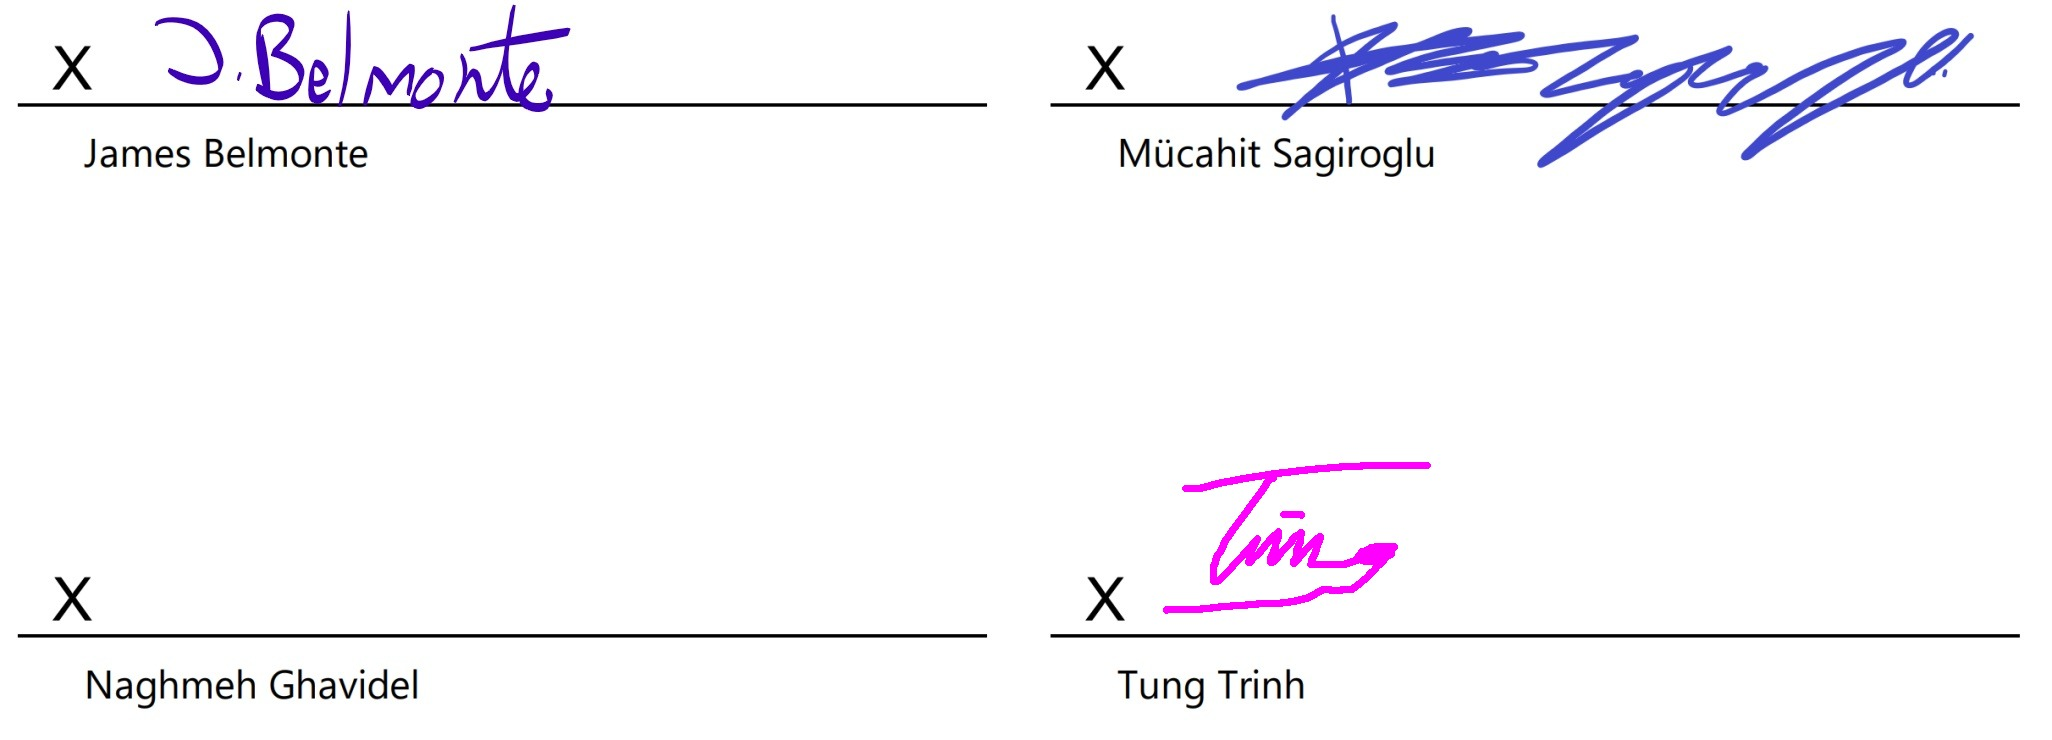
\includegraphics[width=1\linewidth]{Bilder/unterschrift}
\end{figure}

%Inhaltsverzeichnes & Abbildungsverzeichnis & Tabellenverzeichnis
\tableofcontents
\listoffigures
\listoftables
\lstlistoflistings
%ABKÜRZUNGSVERZECIHNIS FEHL!!!!!!!!!!!!!!!!!!!!!!!!!!!!!!!!!!!!!!!!!!!!!!!!!!!!!!!!!!!!!!

%Aktivierung arabische Seitenzahlen
\mainmatter % Seite fängt mit 1 an



%Kapitel: Einleitung
\chapter{Abstract}\label{ch:intro}
Der vorliegende Projektbericht dient als Dokumentation des Informatikprojekts „Software-Defined Network mit OpenFlow“ an der Frankfurt University of Applied Sciences im Bachelorstudiengang Informatik im Wintersemester 2021/2022.\par
Das Aufkommen des Internets hat eine Revolution in der Informationstechnologie geschaffen. Durch eine neue Art der Kommunikation kann der Mensch auf nationaler wie auch auf internationaler Ebene effizienter und effektiver Informationen weitervermitteln. Dies bildet die Grundlage für die heutige Wissensökonomie. \par
Die traditionelle Netzwerkarchitektur ist jedoch seit einem halben Jahrhundert unverändert geblieben und wird für die Geschäftsanforderungen von Unternehmen, Netzwerkbetreibern und Endbenutzern zunehmend ungeeignet. Gegenwärtig werden die Geschäftsanforderungen von Unternehmen immer komplexer und die Anwendungsvielfalt der Endbenutzer nimmt zu, was zu unterschiedlichen Anforderungen der Benutzer an Verbindungsnetzwerke führt. Das Netzwerk muss auf sich schnell ändernde Parameter von Latenz, Bandbreite, Routing, Sicherheit und so weiter (usw.) entsprechend den Anforderungen der Anwendungen reagieren \cite{case}.\par
In den letzten Jahren hat die dramatische Zunahme der Netzwerkkomplexität Schwierigkeiten bei der traditionellen Netzwerkadministration mit sich gebracht. Das Konfigurieren von Computernetzwerksystemen unter Verwendung vordefinierter Richtlinien, das Rekonfigurieren von Netzwerken, um auf Änderungen zu reagieren, die Fehlerkorrektur und der Lastausgleich sind zu gewaltigen Aufgaben geworden. Wenn die Parameter des Netzwerks neu konfiguriert wurden, musste jedes Gerät manuell vollständig neu konfiguriert werden, anstatt einfach nur den Teil der Steuerungsebene zu ändern (vgl. Kim/Feamster 2013: 114f). Dies führte zu einem revolutionären Wandel in der Netzwerktechnologie durch die Zentralisierung der Netzwerkadministration. Seitdem wurde das Konzept des Software-Defined Network (SDN) geboren \cite[114-115]{improve}. 


\section{Software-defined Networking}\label{sdn}
asd
\subsection{Einleitung von James}\label{einl-james}
asddsa
\subsection{Einleitung von Naghmeh}\label{einl-naghmeh}
asddsa
\subsection{Einleitung von Tung}\label{einl-tung}
asddsa
\subsection{Einleitung von Mücahit}\label{einl-müco}
asddsa

\section{Motivation}
Das Modul “Informatik Projekt” wird im 5. Semester des Bachelorstudiengangs Informatik durchgeführt. Nach erfolgreichem Abschluss des Moduls sollten Studierende gewisse Kompetenzen erlernt haben, wie beispielsweise den Software-Engineering Prozess planen und durchführen, als auch auf einem vertieften Niveau gemeinsam programmieren zu können. Außerdem sollten Studierende fähig sein, gemeinsam ein Team zu bilden und einen selbsterstellten Zeitplan einzuhalten sowie auf einem technisch hohen Niveau zu kommunizieren, um als Team auf Ergebnisse zu kommen. Falls unerwartete Komplikationen sowohl technischer als auch sozialer Art entstehen, sollte als Team diese Hürde überwunden werden. Infolgedessen entstand dieser Projektbericht, der als Projektergebnis und als Dokumentation dient, um die erlernten Kompetenzen widerzuspiegeln.\par
Durch das Thema “Software-Defined Networking mit Openflow” konnte Freizeit mit Studium verbunden werden, da viele selbsterlernte Kenntnisse und Vorkenntnisse aus anderen Modulen praktisch angewendet werden konnten. Zugleich dient die Dokumentation durch ausführliche Erklärungen und Abbildungen auch als Tutorial, dass den Einstieg in das Thema SDN durch Praxis vereinfachen soll.
\section{Problemstellung}
Innerhalb des Informatikprojekts muss sich folgendes Szenario vorgestellt werden:\par
Ein Unternehmen plane eine Netzwerkkommunikation zwischen vier Standorten mittels Sofware-Defined Networking Funktionen. Die Hauptverwaltung befinde sich in Frankfurt am Main, die drei weiteren Niederlassungen seien in München, Berlin, Hamburg. Zudem sollte jede Lokation einen Asymmetric Digital Subscriber Line Zugang (ADSL) zum Internet haben.\par
Darüber hinaus müssen im Netzwerk bestimmte Funktionen und Aufgaben realisiert werden. Es solle nicht nur für jede Lokation jeweils ein privater IP-Adressenbereich genutzt werden, sondern auch ein Netzwerkplan vom gesamten Netzwerk erstellt werden. Außerdem solle jede Kommunikation zwischen den einzelnen Lokationen über eine Virtual Private Network Verbindung (VPN) laufen, somit sei der gesamte Datenverkehr über das Internet und zwischen den Lokationen verschlüsselt. Anschließend müsse ein Service-Provider gefunden werden, der die gewünschte Konfiguration und Anforderungen realisiere. Jedoch sollen der Preis und die benötigte Bandbreite nicht nur für den Internetzugang, sondern auch für die Wide Area Network-Verbindungen (WAN) beachtet und verglichen werden. Ebenfalls solle durch SDN sowohl eine Network Address Translation-Firewall-Funktion (NAT) als auch eine Webproxy-Funktion in allen Lokationen implementiert werden. Ergänzend dazu solle mithilfe des SDN-Controllers sowohl eine graphische Darstellung der Netzwerkstruktur durch einen Topologieviewer realisiert werden als auch eine Monitoring-Lösung. Zudem müsse eine Quality of Service -Funktion implementiert werden, die genügend Bandbreite für Audio beziehungsweise (bzw.) Video-Konferenzen habe, auch wenn diese über die WAN-Verbindung mit Symmetric Digital Subscriber Line (SDSL) 20 Megabit begrenzt sei. Anschließend wird ein weiteres Szenario beschrieben:\par
“Für eine Spezialanwendung muss eine Software in Berlin wichtige Daten an einem Server in der Zentrale senden, dazu kann diese Software über die API mit dem Controller kommunizieren und diesem dies mitteilen. Dadurch wird der Controller nun alle Knoten auf diesem Weg durchs Netzwerk anweisen, diesen Flow zu priorisieren und alle anderen Datenströme zu drosseln.” 
Schließlich sollen die Netzwerkfunktionen Hub (Repeater), Bridge, Layer-2-Switch, Layer-3-Switch, Dynamic Host Configuration Protocol (DHCP) und Domain Name System (DNS) analysiert und realisiert werden.\par
In Kapitel 3 wird für die Implementierungen der Netzwerk Funktionalitäten Screenshots von Mininet in VirtualBox gezeigt, die als Nachweis der einzelnen Funktionalitäten dienen sollen.


\section{Aufbau der Arbeit}
In Kapitel 2 dieser Projektarbeit wird über das generelle Vorgehen in dem Projekt geschrieben. Nach einer kurzen Vorstellung unseres Projektziels, wird das konkrete Vorgehen innerhalb der Gruppe erläutert. Weiterhin wird sowohl über die Festlegung der Meilensteine, als auch über die genutzten Werkzeuge eingegangen. In Kapitel 3 wird die Projektdurchführung erklärt und in den Unterkapiteln werden die erreichten Ergebnisse vorgestellt, die auch die einzelnen Thematiken der jeweiligen Funktionalitäten ergänzen. Anschließend dient Kapitel 4 mit einer kurzen Analyse aller Ergebnisse, als auch eine kritische Betrachtung der Projektanforderung, als Auswertung und Selbstreflektion, was im Rahmen der Projektarbeit nicht funktionierte und umgesetzt werden konnte, in Bezug auf Netzwerkanforderungen, sowie intern zwischen allen Gruppenmitgliedern. Kapitel 5 bildet mit dem Fazit einen Ausblick in die mögliche Zukunft für SDN.


\chapter{Projekt}
\section{Projektziel}
Ziel des Projekts war es, ein Netzwerk für ein Unternehmen mit vier Lokationen aufzubauen. Dabei war es besonders wichtig, dass das gesamte Netzwerk mit SDN Funktionen realisiert wurde.\par
Ein stabiles Netzwerk vom ersten Tag an wird die Grundlage für den Erfolg von Unternehmen sein. Damit Unternehmen gut funktionieren, muss auch das Netzwerksystem gut funktionieren. Das Netzwerk arbeitet mit der richtigen Kapazität und bringt Effizienz. Die Aufgabe war es, ein gutes stabiles Netzwerk aufzubauen, dass zu 100 Prozent bei Datenverkehr funktionierte und unerwartete Sicherheitsprobleme vermeidete.\par
Das Netzwerksystem musste eng verwaltet und überwacht werden. Zudem musste es leicht unterstützt werden, um Probleme auf die effektivste Weise behandeln und beheben zu können. Es war zwingend erforderlich, dass das Netzwerksystem sicher und verschlüsselt war. Denn Unternehmensdaten sind das Wichtigste. Bei der Netzwerksicherheit ging es auch um den Schutz von Unternehmensressourcen. Je nach Verwendungszweck und Anzahl der Nutzer sollten genügend Bandbreite zur Verfügung gestellt werden.\par
Im Laufe des Projektberichtes werden die erfolgreichen sowie erfolglosen Ergebnisse des Projekts dokumentiert und dargestellt. Am Ende des Projektes wird ein lauffähiges Produkt entstehen, dass alle benötigten Funktionalitäten erfüllt.  

\section{Vorgehen}
Angemessene Aufgabenverteilung im Kollektiv, brachte viele Vorteile für die Arbeitssituation und den Teammitgliedern. Die Nutzung der maximalen Kapazität jedes Teammitglieds war ein effektiver Weg, um die Arbeitseffizienz zu verbessern.\par
Um die Wünsche und Fähigkeiten jedes einzelnen Mitglieds zu verstehen, wurden Gespräche und Diskussionen frühzeitig durchgeführt. Die Zuweisung von Aufgaben, die der Produktivität jeder Person entsprachen, half den Mitgliedern, effektiver und mit einem angenehmeren Geist zu arbeiten. Den Mitgliedern wurden bestimmte Aufgaben mit Fristen zugewiesen. Es wurde jede Woche ein permanentes Treffen über Discord gehalten. Spontane Treffen konnten mit dem höchsten Geist und der höchsten Konzentration ebenfalls durchgeführt werden.\par
Die Analyse von Aufgabenzuweisungen war wichtig, um zu verstehen, was getan werden muss und welche Tools notwendig seien. Der Wissensaustausch half den Mitgliedern, sich Wissen sofort anzueignen und effektiv zu nutzen. Nach einer erfolgreichen Analyse begann unser Team mit der Ausarbeitung eines Plans. Die Arbeit wurde vom Projektleiter aufgeteilt und kontrolliert.

\section{Festlegen von Meilensteinen}
In dem ersten Treffen der Gruppe wurde entschieden, drei zentrale Meilensteine zu definieren (siehe Abbildung \ref{milestones}). Grund dafür sei, einen klaren Faden in der Projektarbeit zu konstruieren, um mit der Menge an Informationen strukturiert umgehen zu können. Die Meilensteine wurden mithilfe der Aufgabenstellungen konkretisiert:

\begin{figure}[htbp]
 \centering
 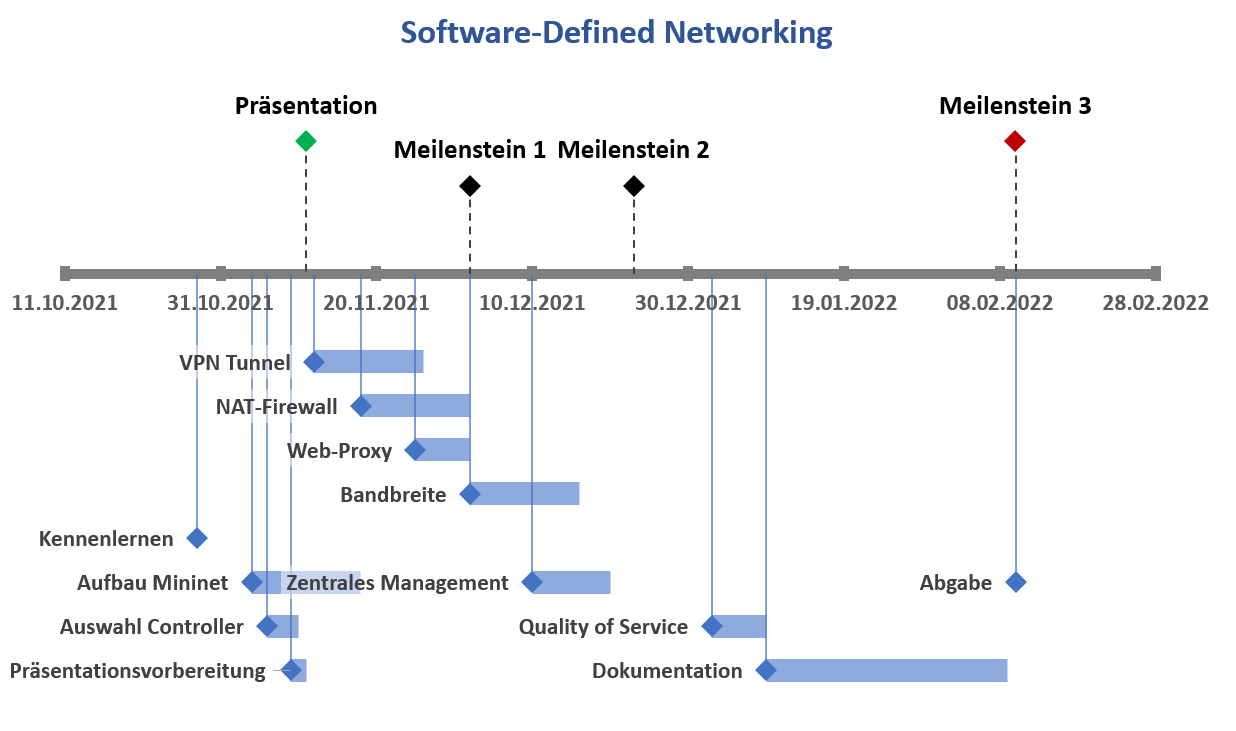
\includegraphics[width=1.0\textwidth]{Bilder/meilensteine}
 \captionsetup{justification=centering,margin=2cm}
 \caption{Zeitplan des Projektes}
 \label{milestones}
\end{figure}

\textbf{Meilenstein 1}
\begin{itemize}
 \item Erstellung eines Netzwerkplans für das gesamte Netzwerk
 \item Kommunikation zwischen Lokationen soll über eine VPN Verbindung realisiert werden
 \item Produktauswahl bei einem ISP zur Realisierung des Netzwerkes
 \item Implementierung einer NAT-Firewall-Funktion in allen Lokationen
 \item Deadline: 02.12.2021
\end{itemize}

\textbf{Meilenstein 2}
\begin{itemize}
 \item Implementierung einer Webproxy-Funktion für den Internet-Zugang in den einzelnen Lokationen
 \item Implementierung eines Topologie-Viewers und einer Monitoring-Lösung
 \item Implementierung einer Quality of Service Funktion für Audio- und Videokonferenzen
 \item Deadline: 23.12.2021
\end{itemize}

\textbf{Meilenstein 3}
\begin{itemize}
 \item Priorisierung von einem Datenflow mithilfe des Controllers
 \item Analyse und Umsetzung der Netzwerkfunktionen von Hub, Bridge, Layer-2-Switch, Layer-3-Switch, DHCP und DNS
 \item Deadline: 10.02.2022
\end{itemize}

Durch gängige IT-Projektmanagementmethoden, wie beispielsweise die Scrum-Methode, konnten frühzeitig Ergebnisse erzielt werden. Infolgedessen gab es am Ende der Projektarbeit mehr Zeit, um über Kleinigkeiten zu reflektieren.

\section{Verwendete Werkzeuge}
Im Folgenden werden die für die Implementierung und Evaluierung verwendeten Hardware- und Softwareumgebungen kurz beschrieben.\par
Dieses Projekt wurde auf VirtualBox Oracle VM Version 6.1 durchgeführt. Unter der Verwaltung von VirtualBox wurde Mininet-Emulator Version 2.3 und Floodlight Controller Version 1.2 installiert. Zur Ausführung von Programmen zur Evaluation wurde außerdem Python3 installiert. Weitere Programme sind auch installiert und sie werden im Ablauf von Kapitel 3 bekannt gegeben und ausführlicher erklärt.

\subsection{Mininet}
Der Mininet-Emulator implementiert die Verbindung zwischen Switches und Controllern. Diese ermöglicht es Entwicklern, die an der Erstellung und dem Testen von Controller-Ressourcen interessiert sind, Mininet zur Durchführung ihrer Simulationen zu nutzen.

\subsubsection{Einführung}
Mininet ist ein Netzwerk Emulator, mit der Netzwerke simuliert werden können. Bei Mininet handelt es sich um eine kostenlose Open-Source-Software, die die virtuelle Maschine und dem Controller die Recherche in SDN und OpenFlow ermöglicht. Mininet ermöglicht eine sehr groß angelegte Topologie, wodurch ein Netzwerk von Hosts, Switches, virtuellen Links und einem Controller erstellt wird. Das Ausführen von Tests mit den Komponenten ist unkompliziert und kann über Python-Schnittstelle erledigt werden. Benutzer können ihre eigene Netzwerktopologie-Struktur nach ihren eigenen Bedürfnissen aufbauen.

\subsubsection{Funktionalität}
Mininet:
\begin{itemize}
 \item stellt ein einfaches Netzwerk Testbed dar, welches aber auch gleichzeitig günstig ist. Da der OpenFlow Switch in Mininet alle Eigenschaften wie ein echter OpenFlow Switch hat, ist die Anwendung von einem Netzwerkemulator mit Mininet praktisch sinnvoll.
 \item ermöglicht das Debuggen und Ausführen von Tests größerer Netzwerke mithilfe von Command Line Interface (CLI).
 \item unterstützt das Einrichten beliebiger benutzerdefinierter Diagramme. Die Anwendungen im Mininet können im echten Netzwerk realisiert werden, ohne dass der Code geändert werden muss.
 \item bietet eine benutzerfreundliche und erweiterbare Python-API.
 \item ermöglicht mehreren gleichzeitigen Entwicklern, unabhängig voneinander an derselben Topologie zu arbeiten.
 \item ermöglicht komplexe Topologietests, ohne dass ein physisches Netzwerk verkabelt werden muss.
\end{itemize}

\subsubsection{Nachteile}
Aktuell ist Mininet nur unter Linux lauffähig. Nutzer eines anderen Betriebssystems müssen auf Linux entweder durch Simulierung oder Installation zurückgreifen. Zudem könnte der Sourcecode effizienter und sauberer implementiert werden.\par
Mininet schreibt Ihren OpenFlow-Controller nicht für Benutzer. Wenn Benutzer benutzerdefiniertes Routing- oder Schaltverhalten benötigen, müssen Benutzer einen Controller mit den erforderlichen Funktionen finden oder entwickeln.\par
Standardmäßig ist Mininet-Netzwerk von Local Area Network (LAN) und vom Internet isoliert - das ist normalerweise eine gute Sache! Benutzer können jedoch das NAT-Objekt und/oder die Option --nat verwenden, um Ihr Mininet-Netzwerk über Network Address Translation mit Ihrem LAN zu verbinden. Benutzer können Ihrem Mininet-Netzwerk auch eine echte (oder virtuelle) Hardware-Schnittstelle hinzufügen (siehe Beispiele/hwintf.py für Details).\par
Standardmäßig teilen sich alle Mininet-Hosts das Host-Dateisystem und den PID-Speicherplatz. Das bedeutet, dass Benutzer möglicherweise vorsichtig sein müssen, wenn sie Daemons ausführen, die eine Konfiguration in /etc erfordern, und Benutzer müssen darauf achten, dass sie nicht versehentlich die falschen Prozesse beenden. \par
Im Gegensatz zu einem Simulator hat Mininet keine starke Vorstellung von virtueller Zeit. dies bedeutet, dass Timing-Messungen auf Echtzeit basieren und dass Ergebnisse schneller als Echtzeit (z. B. 100-Gbit/s-Netzwerke) nicht einfach emuliert werden können.

\subsubsection{Komponenten}
Ein Mininet-Netzwerk besteht aus den folgenden Komponenten:
\begin{itemize}
 \item \textbf{Link:} Links sind virtuelle Ethernets, die zwei virtuelle Schnittstellen verbinden. Jeder Link verhält sich für das gesamte System wie ein echter funktionsfähiger Ethernet-Anschluss. Die Datenrate jedes Links wird von Linux Traffic Control (TC) festgelegt.
 \item \textbf{Hosts:} Ein emulierter Host ist eine Reihe von Prozessen auf Benutzerebene, die in einen Netzwerk-Namespace verlagert wird. Netzwerk-Namespaces bieten Prozessgruppen privaten Besitz von Schnittstellen, Ports und Routing-Tabellen.
 \item \textbf{Switch:} Mininet verwendet Open vSwitches, die im Kernelmodus ausgeführt werden, um Pakete zwischen verschiedenen virtuellen Netzwerkschnittstellen auszutauschen. Open vSwitches sind OpenFlow-fähig und bieten die gleiche Semantik für das Senden von Paketen wie einen realen Switch.
 \item \textbf{Controller:} Ein Controller ist in der Mininet-Simulation ein Knoten, der einen OpenFlow-Controller darstellt. Mininet bietet die Möglichkeit einen internen oder externer Controller zu benutzten. Für den externen Controller wird die IPv4-Adresse und der Port benötigt.
\end{itemize}


\subsubsection{Installation}
Mininet kann auf verschiedene Weisen installiert werden. In unserer Arbeit wurde die Option: Native Installation from Source ausgewählt. Die Installation wird Schritt für Schritt aufgeführt:
\begin{itemize}
\item[1.] Git wird über das Linux-Terminal installiert
\end{itemize}
\colorbox{CadetBlue}{\textcolor{white}{\textbf{\textsf{\$ sudo apt-get install git}}}}
\begin{itemize}
\item[2.] Über das git Kommando wird die aktuellste Version von Mininet installiert
\end{itemize}
\colorbox{CadetBlue}{\textcolor{white}{\textbf{\textsf{\$ git clone git://github.com/mininet/mininet}}}}
\begin{itemize}
\item[3.] Mit install.sh die Installation starten
\end{itemize}
\colorbox{CadetBlue}{\textcolor{white}{\textbf{\textsf{\$ sudo mininet/util/install.sh -a}}}}

\subsubsection{Aufbau}
Durch die Eingabe von dem Befehl \textit{\textbf{sudo mn}} wird ein Standardnetzwerk mit zwei Hosts, einer Switch und einem Controller gestartet (siehe Abbildung \ref{sudomn}).

\begin{figure}[htbp]
 \centering
 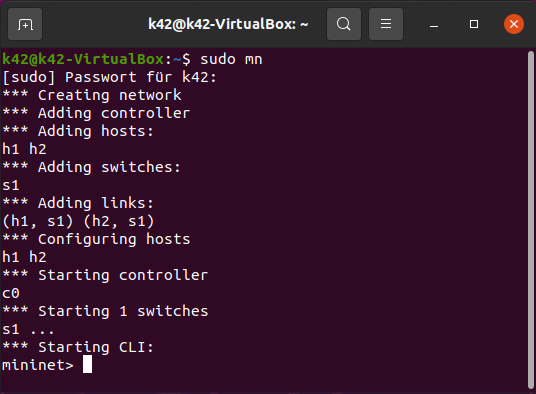
\includegraphics[width=0.5\textwidth]{Bilder/sudomn}
 \captionsetup{justification=centering,margin=2cm}
 \caption{Erstellung eines Standardnetzwerkes mit Mininet}
 \label{sudomn}
\end{figure}

\subsection{Floodlight}
Floodlight ist ein sogenannter Controller zur Steuerung einer oder mehreren programmierbaren Switches. Die Kommunikation zwischen Switch und Controller erfolgt über ein Kommunikationsprotokoll namens OpenFlow. Die Kontrolle der Switches erfolgt entweder durch Programmierung oder einer vom Controller zur Verfügung gestellten und benutzerfreundlichen Schnittstelle.

\subsubsection{Einführung}
In den letzten Jahren wurde eine Vielzahl unterschiedlicher SDN-Controller entwickelt. Aus diesem Grund gibt es mittlerweile eine riesige Auswahl an SDN-Controllern für die breit gefächerten Einsatzzwecke, wo unteranderem OpenDaylight, Ryu, POX, NOX und Floodlight dazugehören. Mit allen Controllern sind alle Projektziele der Projektarbeit erzielbar.\par
Floodlight wurde als Controller ausgewählt, da einige Punkte und das daraus resultierende Gesamtprodukt die Gruppe überzeugen konnte. Dazu gehört unteranderem die einfache und gut beschriebene Installation. Die moderne Webbenutzeroberfläche und die verständliche, gut dokumentierte REST-API sind sehr benutzerfreundlich und leicht zu verstehen. Daraus resultiert auch die Option, die REST-API über ein Python-Skript zu benutzen. Die Einbindung des Floodlight-Controllers in Eclipse ermöglicht die Implementierung, Untersuchung und das Debuggen verschiedenster Controller-Funktionen. Die gute Dokumentation des in Java geschriebenen Controllers und einige mit der Installation mitgelieferten Beispielanwendungen geben einem Entwickler einen guten Start zur Entwicklung von Netzwerkfunktionen.

\subsubsection{Funktionalität}
Die Funktionalitäten des Floodlight-Controllers unterscheiden sich anhand der Ausführung und der Implementierung. Funktionen können über die Webbenutzeroberfläche per Eingabe ausgeführt werden (siehe Abbildung \ref{webui}). Das Einstellen der Switch-Firewall und der Access Control List sind zwei dieser Funktionen. Nach Aktivierung der Firewall werden alle Pakete, die nicht in der Liste eingetragen sind, fallen gelassen. Die Access Control List arbeitet ähnlich wie die Firewall, wohingegen nur eine Liste mit erwünschten und nicht erwünschten Quellen existiert. Die Quellen werden anhand der Paket-Informationen angegeben. Bei einem Treffer wird die Quelle je nach Einstellung zugelassen oder verweigert. Folglich verweigert die Firewall jegliche Verbindung nach Aktivierung, wohingegen die Access Control List nur bestimmte Zugriffe auf ein Netzwerk zulässt oder ablehnt. Auf der Webbenutzeroberfläche sind Informationen zu dem vom Controller gesteuerten Netzwerk einsehbar. Dazu gehört die Anzahl der Switches, Hosts und Links sowie der verbrauchten Ressourcen des Controllers und der Netzwerktopologie. Die Statistikfunktion des Controllers kann auf der Benutzeroberfläche aktiviert werden. Dieser dient zur ausführlichen Weiterverarbeitung und der Anzeige der vom Controller gesammelten Statistik. Dazu gehören die Flow, meter, queue, aggregate, table und port Statistiken. Die Sammlung benutzerdefinierter Statistiken sind ebenfalls möglich und müssen vom Entwickler nachimplementiert werden. Über die REST-API können sogenannte Flows eingetragen werden, die zur Steuerung des Netzwerkes beitragen. Dabei können Datenpakete modifiziert, zwischengespeichert und umgeleitet werden.

\begin{figure}[htbp]
 \centering
 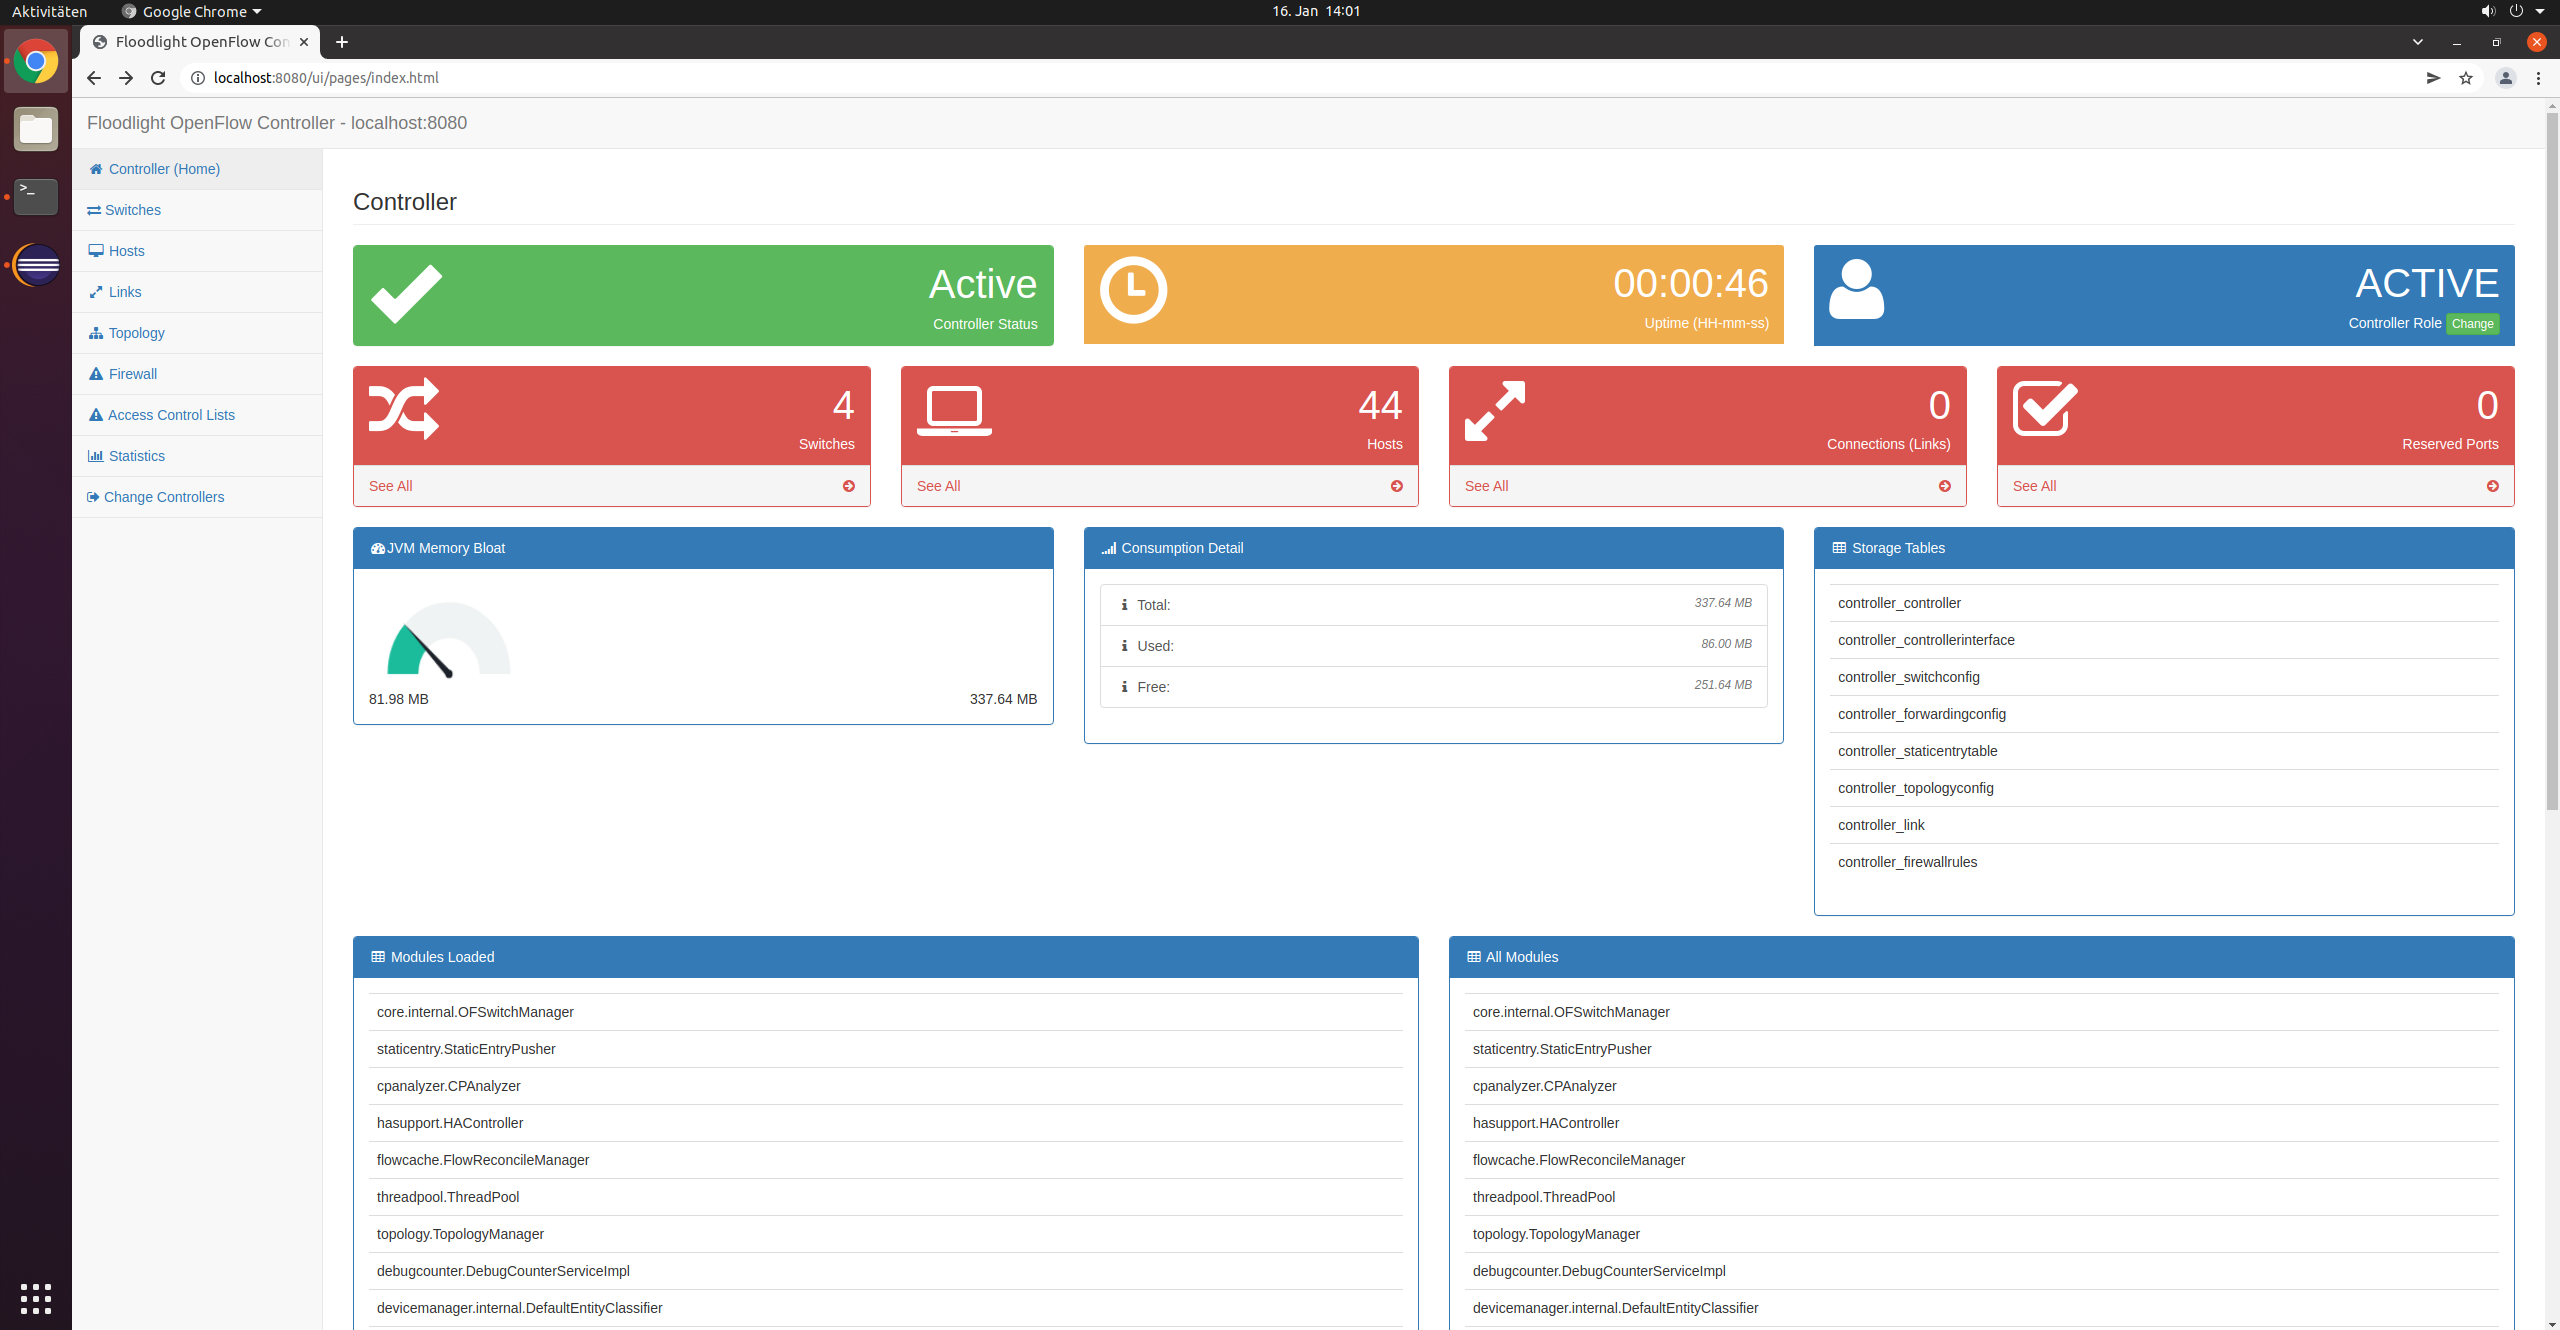
\includegraphics[width=1.0\textwidth]{Bilder/webui}
 \captionsetup{justification=centering,margin=2cm}
 \caption{Webbenutzeroberfläche vom Floodlight-Controller}
 \label{webui}
\end{figure}


\subsubsection{Nachteil}
Das ganze Netzwerk ist betroffen, wenn Floodlight ausfällt oder nicht erreichbar ist. Dieser Single Point of Failure gilt für alle Controller und stellt ein Risiko für Netzwerke, die eine hohe Verfügbarkeit und Zuverlässigkeit fordern. Die Wartung und Konfiguration eines Controllers für komplexe Netzwerkstrukturen erfordern viele geschulte Angestellte.

\subsubsection{Komponenten}
Mit der Installation von Floodlight kommen sogenannte Module zum Einsatz. Die meisten der Module sind bereits aktiviert und stellen bestimmte Funktionen zur Verfügung. Einer davon ist die Learning Switch, welcher für die Speicherung der Routen zu den Hosts zuständig ist. Wenn ein Host einen anderen Host im gleichen Netzwerk erreichen will und der Switch die Route nicht kennt, wird ein Broadcast ausgeführt, der die Anfrage auf allen Ports ausgibt. Wenn der Host antwortet, speichert der Switch die MAC-Adresse des jeweiligen Hosts ab und muss somit keinen Broadcast durchführen. Weitere Beispielmodule wären der Load Balancer und der Topology Manager. Der Load Balancer sorgt für einen Ausgleich des Datenverkehrs im gesamten Netzwerk. Der Topology Manager stellt die Netzwerktopologie über die Webbenutzeroberfläche grafisch dar. Es existieren noch weitere Module, wobei auch eigene programmiert werden können.

\subsubsection{Installation}
Die Installation des Floodlight-Controllers kann auf den Betriebssystemen Linux, Mac oder Windows erfolgen. Es wird das Java Development Kit 8, Maven, Git, build-essential und das Python Development Paket benötigt. Da Floodlight in Java geschrieben wurde, wird auch zur Ausführung Java verwendet. Maven wird zum sogenannten Builden benutzt, bei dem die Software Floodlight aus mehreren Dateien zusammengestellt wird. Das Python Development Paket wird zur Ausführung und Git zum Herunterladen von Floodlight vorausgesetzt. Build-essential werden zum Kompilieren einiger Software verwendet. Im Folgenden wird die Installation auf Linux Schritt für Schritt erklärt. Befehle müssen im Linux-Terminal zeilenweise eingegeben werden.

\begin{itemize}
\item[1.] Alle benötigten Abhängigkeiten installieren.
\end{itemize}
\colorbox{CadetBlue}{\textcolor{white}{\textbf{\textsf{\$ sudo apt-get install build-essential git maven python-dev openjdk-8-jdk}}}}
\begin{itemize}
\item[2.] Java Compiler als Alternative festlegen. Befehl eingeben und JDK 8 Auswählen.
\end{itemize}
\colorbox{CadetBlue}{\textcolor{white}{\textbf{\textsf{\$ sudo update-alternatives --config javac}}}}
\begin{itemize}
\item[3.] Programmcode per Github herunterladen und aktualisieren
\end{itemize}
\colorbox{CadetBlue}{\textcolor{white}{\textbf{\textsf{\$ git clone git://github.com/floodlight/}}}}\\
\colorbox{CadetBlue}{\textcolor{white}{\textbf{\textsf{\$ floodlight.git}}}}\\
\colorbox{CadetBlue}{\textcolor{white}{\textbf{\textsf{\$ cd floodlight}}}}\\
\colorbox{CadetBlue}{\textcolor{white}{\textbf{\textsf{\$ git submodule init}}}}\\
\colorbox{CadetBlue}{\textcolor{white}{\textbf{\textsf{\$ git submodule update}}}}
\begin{itemize}
\item[4.] Floodlight Ordnerrechte zuweisen und Builden
\end{itemize}
\colorbox{CadetBlue}{\textcolor{white}{\textbf{\textsf{\$ cd ..}}}}\\
\colorbox{CadetBlue}{\textcolor{white}{\textbf{\textsf{\$ sudo chown -hR Benutzername:Gruppenname floodlight/}}}}\\
\colorbox{CadetBlue}{\textcolor{white}{\textbf{\textsf{\$ cd floodlight/}}}}\\
\colorbox{CadetBlue}{\textcolor{white}{\textbf{\textsf{\$ mvn package -DskipTests}}}}
\begin{itemize}
\item[5.] Floodlight im Terminal ausführen (siehe Abbildung)
\end{itemize}
\colorbox{CadetBlue}{\textcolor{white}{\textbf{\textsf{\$ java -jar target/floodlight.jar}}}}

Es besteht die Möglichkeit, den Floodlight Controller mithilfe von Eclipse zu starten, somit muss Floodlight nicht im Terminal ausgeführt werden. Außerdem ist Floodlight durch die Entwicklungsumgebung Eclipse leichterer auszuführen und eine Bearbeitung ist übersichtlicher. Zudem hat man eine schnelle Übersicht vom kompletten Conroller, da alle Klassen in einem Eclipse Ordner einzusehen sind. Mit sudo mvn package –Declipse werden mehrere Dateien erstellt. Mit den neu erstellten Dateien kann ein neues Eclipse Projekt importiert werden. Anschließend wird Eclipse gestartet und eine neue Arbeitsumgebung erstellt. \textit{\textbf{File -> import -> General -> Existing Projects into Workspace}} und auf \textit{\textbf{Next}} klicken. Von \textit{\textbf{Select root directory}} auf \textit{\textbf{Browser}} klicken und Verzeichnis das Floodlight enthält auswählen. Das Projekt mit \textit{\textbf{finish}} ausführen und damit sollte Floodlight auf Eclipse importiert sein.\par
Um Floodlight auf Eclipse auszuführen, wählt man \textit{\textbf{run configuration}} aus, rechts klickt auf \textit{\textbf{java application}} und \textit{\textbf{new}}. Anschließend wird die neue Java Application \textit{\textbf{FloodlightLaunch}} genannt, es nutzt das Projekt Floodlight und \textit{\textbf{net.floodlight.controller-\\.core.Main}} in der Main-Klasse. Nachdem dies konfiguriert wurde, kann das Programm in Eclipse ausgeführt werden.


\subsubsection{Aufbau}
Nach erfolgreicher Installation und Ausführung von Floodlight läuft der Controller standardmäßig auf Port 6653. Im Terminal werden alle informativen Ereignisse ausgegeben. Um den Controller zu stoppen, wird die Tastenkombination Steuerung und C gleichzeitig gedrückt (siehe Abbildung \ref{floodlight}).

\begin{figure}[htbp]
 \centering
 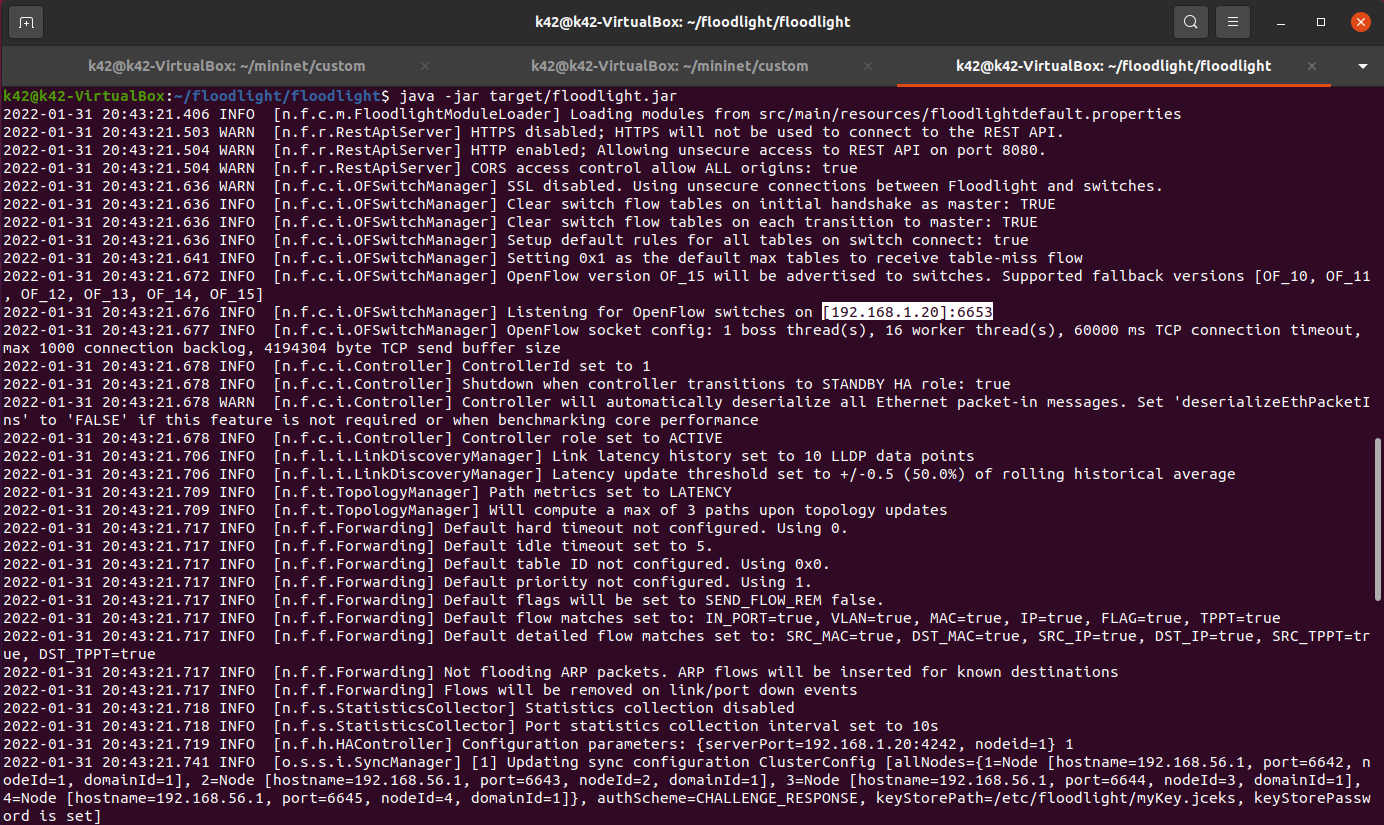
\includegraphics[width=1.0\textwidth]{Bilder/floodlight}
 \captionsetup{justification=centering,margin=1cm}
 \caption{Ausführung von Floodlight über den Linux-Terminal}
 \label{floodlight}
\end{figure}

\newpage
\subsection{Ergebnis}


\setlength{\intextsep}{0pt}
\setlength{\columnsep}{15pt}
\begin{wrapfigure}{R}{0.5\textwidth}
    \centering
    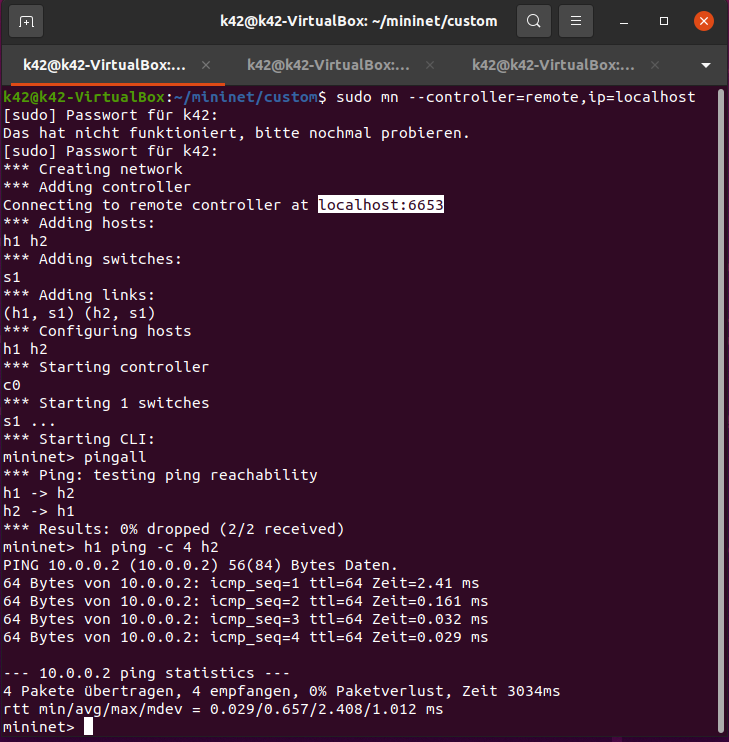
\includegraphics[width=0.5\textwidth]{Bilder/ping}
    \caption{Mininet Controller Verbindung und Ping-Test}
    \label{ping}
\end{wrapfigure}

Nach der Ausführung von Floodlight, wurde dieser mit einer OpenFlow-fähigen Switch verbunden. Der Switch wurde mit Mininet mit der Angabe des Controllers simuliert. Die Konsole zeigt die erfolgreiche Verbindung mit dem Controller. Die Konnektivität im Netzwerk kann mit dem Befehl \textit{\textbf{pingall}} überprüft werden. Die Konnektivität zwischen Host 1 und Host 2 wird durch den Befehl \textit{\textbf{h1 ping h2}} getestet. Durch Wireshark kann der ausgelöste Datenverkehr betrachtet werden (siehe Abbildung \ref{ping}).



\chapter{Durchführung des Projektes}
Die in Kapitel 1.3 dargestellten Problemstellungen werden in diesem Kapitel behandelt und realisiert. Durch Abbildungen, Code Ausschnitte und Erläuterungen soll die Dokumentation die Vorgehensweise und Überlegungen der Gruppe wiedergeben. 



\section{Netzwerkplan}
\subsection{Vorüberlegung}
Das Netzwerkmodell umfasst:
Mininet: 4 Switches und 40 Hosts erstellen. Diese Switches und Hosts werden verbunden mit unserem Floodlight Controller. 4 Switches repräsentieren 4 Lokationen mit jeweils 10 Hosts. Damit die Hosts und Switches mit dem Internet verbunden werden können, steht 4 Routers da. Router kann man wie ein Gateway betrachten. Anhand von Headern und Weiterleitungstabellen bestimmt der Router den besten Weg zur Weiterleitung der Pakete.
Floodlight Controller: SDN-Controller (SDN-Controller) steuert den Zugriff zwischen Hosts im Netzwerk. Dies wird durch eine Python Datei implementiert

\begin{figure}[htbp]
 \centering
 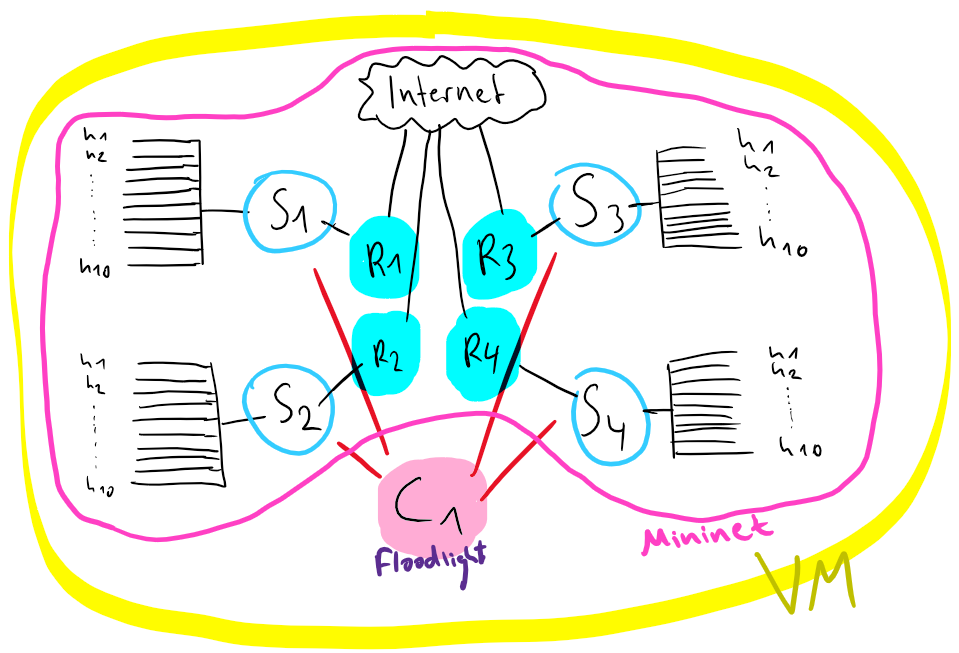
\includegraphics[width=1.0\textwidth]{Bilder/prototyp}
 \captionsetup{justification=centering,margin=2cm}
 \caption{Netzwerkplan unseres Unternehmens}
 \label{networkplan}
\end{figure}

\subsection{Durchführung}


\begin{figure}[htbp]
 \centering
 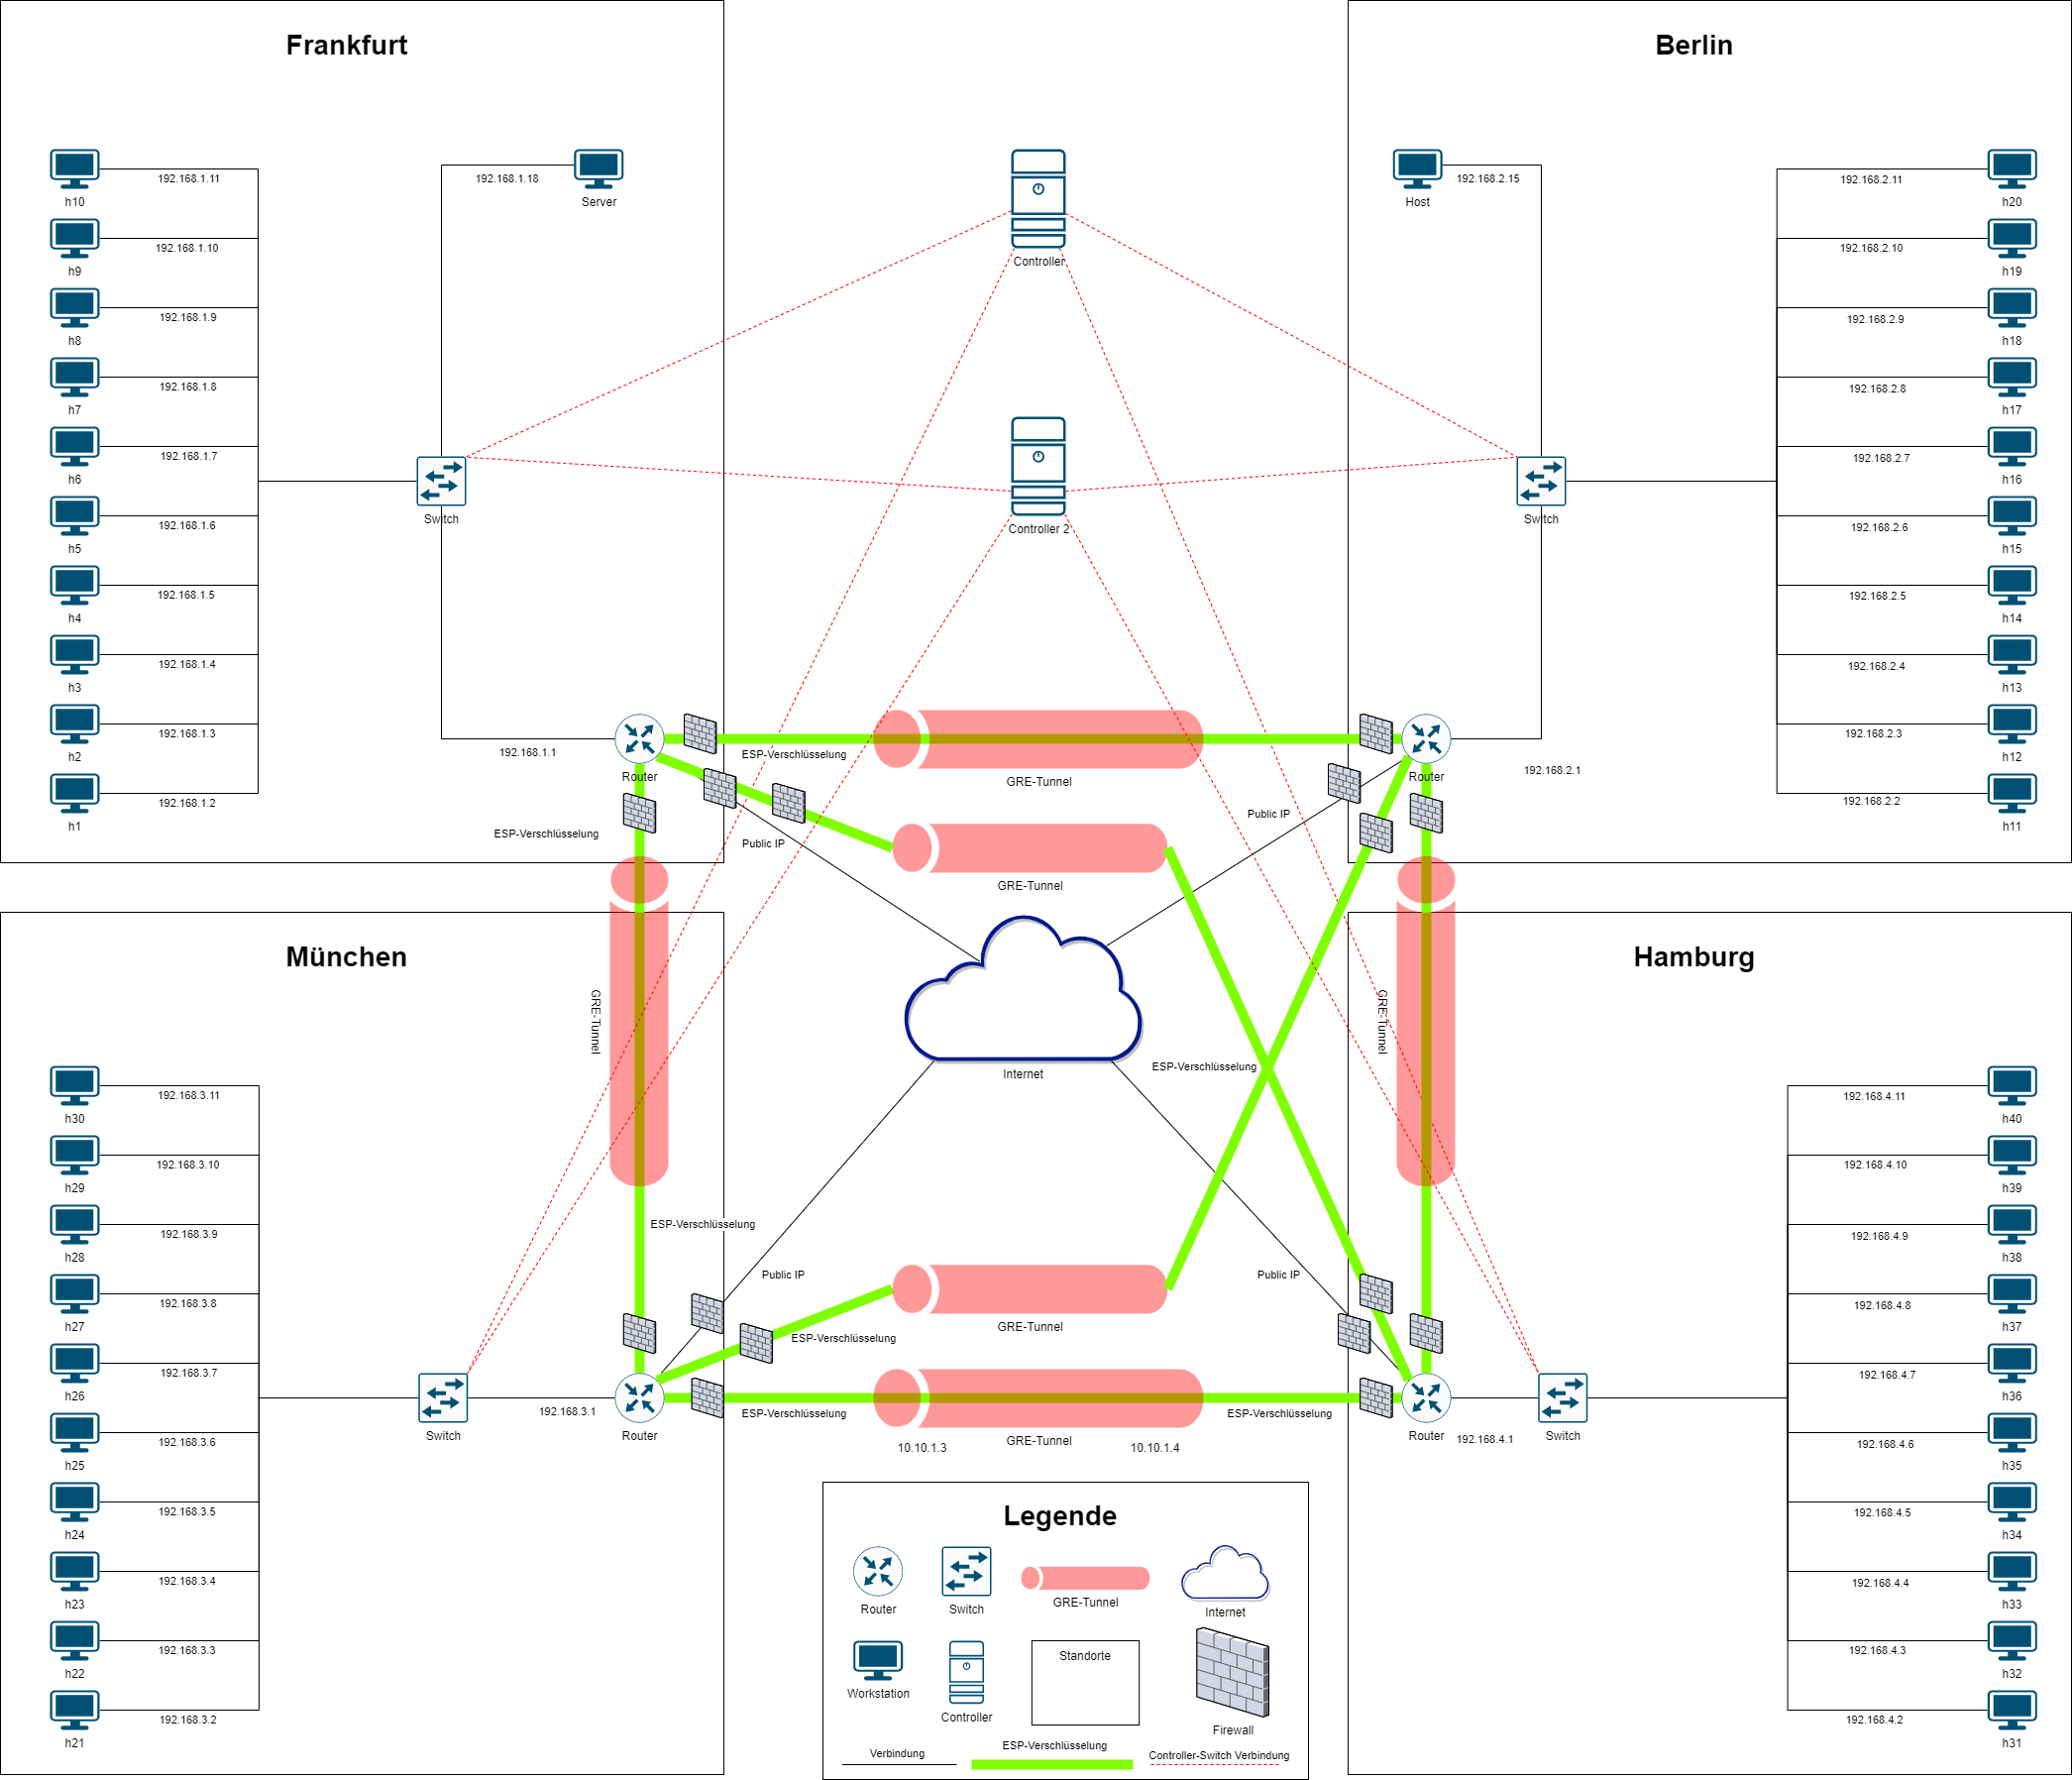
\includegraphics[width=1.0\textwidth]{Bilder/netzwerkplan}
 \captionsetup{justification=centering,margin=2cm}
 \caption{Netzwerkplan unseres Unternehmens}
 \label{networkplan}
\end{figure}

\section{Aufbau des Netzwerkgerüstes in Mininet}
\subsection{Durchführung}
In diesem Abschnitt wird der Aufbau der Simulation über Mininet erklärt.
 
In der Main-Funktion werden die Komponenten eines Netzwerks deklariert und aufgerufen. Das sind eine Topologie, ein Controller mit zugewiesenem Port und ein Mininet Objekt mit der deklarierten Topologie. Anschließend geben wir für unsere Routers Routing-Regeln und Informationen.

\subsection{Aufbau der Topologie}
Der Mininet-Script besteht aus einer Main-Funktion bei der als allererstes mit der von uns definierten Klasse „Netzwerk()“. Und damit zeigen wir wie das Netzwerk beziehungsweise eine Topologie erstellt wird. Die Klasse übernimmt ein Topo-Objekt an dem er mit der in ihm definierten „build()“ Methode die Konfiguration des Netzwerkes vornimmt. 
 
In der „build()“ Methode definieren wir zuerst einen String der den privaten-IP-Bereich der vier Lokationen enthält. Der defaultIP String bleibt in unvollständiger Form „192.168.\%s.1/24“. Somit kann er später durch passende Stellen ersetzt und genutzt werden. Lediglich ist hier im dritten Block ein Platzhalter eingesetzt der beim erstellen der Router in einer Schleife durch die Zahl der Iteration ersetzt wird.
 
Zunächst wird ein leeres Array/Liste unter dem Namen „Routers“ deklariert. Dies wird dann später genutzt und mit den Router-Objekten gefüllt. Später für die Verlinkung der Router mit dem jeweiligen Switch wird die Liste aufgerufen. Für große Anzahl von Router ist die Bedeutung der Liste sehr praktisch.
 
Im nächsten Teil der Klasse Netzwerk, Zeile 35 bis 53 wollen wir die Komponenten des Netzwerks implementieren. Dies ist mit Hilfe einer Schleife mit 4 Durchläufe ausgeführt worden. 4 Durchläufe entsprechen 4 Lokationen, jeweils 1 Switch 1 Router und 10 Hosts.
Dabei wird bei jeder Iteration erst ein Router-Objekt mit der Methode „self.addNode()“ erstellt, bei dem der Name, der private IP-Adressen-Bereich, die MAC-Adresse und benutzerdefinierte Parameter für die Konfiguration, dass der Router IP-Forwarding aktiviert bekommt, übergeben. Danach wird der Router der vorher erstellten Liste eingefügt.
 
Als nächstes wird ein Switch mit der Methode „self.addSwitch()“ erstellt, der nur einen Namen erhält, der anschließend mit der Methode „self.addLink()“ mit dem Router verbunden wird, bei dem die Netzwerkschnittstelle des Router benannt und der private-IP-Adressenbereich vergeben wird.
 
Danach folgt noch eine Schleife, bei der insgesamt n Hosts erstellt und mit dem Switch verbunden werden. Die Hosts erhalten für den jeweiligen privaten-IP-Bereich eine IP, eine MAC-Adresse und die IP des jeweiligen Routers als Standard-Route zugewiesen. 
Nachdem für alle Lokationen der Rumpf erstellt worden ist, stellen wir die Verbindungen zwischen den Routern mit dem Befehl „self.addLink()“ her. Dabei wird jeder Router mit allen anderen Routern verbunden. Dieser Vorgang wird das Internet simulieren, worauf ebenfalls der Tunnel und die Verschlüsselung implementiert wird. Dabei wird der Netzwerkschnittstellen-Name für beide Router und die jeweilige öffentliche-IP-Adresse definiert. Zusätzlich setzen wir per „bw=20“ Befehl die Bandbreite der Leitung auf 20 Megabit, wobei dies die geforderte SDSL-Leitung der Aufgabe sieben darstellen soll. 

\subsection{Controller Implementierung}
Es würde weiter bei der Main-Funktion gehen. Dort initialisieren wir ein RemoteController-Objekt der einen Namen, die Konfiguration um was für einen Controller es sich handelt, die IP-Adresse und den Port, wo er zu erreichen ist, bekommt. Hier ist wichtig zu erwähnen, dass der Controller auf Ubuntu läuft und das der Controller per „localhost“ zu erreichen ist. Hier könnte man ebenfalls den Controller auf einer anderen VM laufen lassen und ihn per Internes Netzwerk verbinden oder auf der echten Welt laufen lassen und ihn per NAT-Verbindung verbinden. Auch besteht noch die Möglichkeit den Controller auf dem Betriebssystem, auf dem Virtualbox läuft, laufen zu lassen und ihn per Host-Only-Adapter zu verbinden. Anschließend wird ein Mininet-Objekt erstellt, bei dem die erstellte Topologie, der erstellte Controller, ein TCLink-Objekt für die Einstellung der Bandbreite der Netzwerkadapter und ein OVSKernelSwitch-Objekt für die Erstellung der Switche als Open vSwitche. Die Open vSwitche nutzen wir später, um den Quality of Service zu implementieren, bei dem wir per ovs-vsctl-Befehle Queues an den Ports der Switche erstellen und die Priorisierung der Pakete vornehmen. 

\subsection{Ergebnis}
Was haben wir dadurch erreicht. Zusammenfassen.
Was ist schief gelaufen?

\section{Verschlüsselung der Netzwerkverbindung zwischen den Lokationen}
Als nächstes folgt in der Main-Funktion die Einrichtung der Tunnel zwischen den Routern beziehungsweise den Lokationen. Dafür baut jeder Router mit jedem Router einen GRE-Tunnel auf, für den wir den Befehl „ip tunnel add Tunnel-Name mode gre local Router-Schnittstelle-des-eigenen-Routers remote Router-Schnittstelle-des-anderen-Routers ttl 255“ bei jedem Router mit der Mininet-Methode „info(net[‚Router-Name‘].cmd(Befehl))“ ausgeben und ausführen. Nachdem die Verbindung definiert wurde fahren wir den Tunnel-Adapter per „ip link set Tunnel-Name up“ hoch. Anschließend geben wir dem Tunnel Adapter mit dem Befehl „ip addr add Tunnel-IP dev Tunnel-Name“ die jeweilige Tunnel IP. Hier ist wichtig zu erwähnen, dass die IP zwischen zwei Lokationen im selben Netzwerkbereich, wie bei der Erstellung und Simulierung des Internets zwischen den Routern, sein muss. Nachdem der Tunnel aufgesetzt worden ist, sind alle Pakete, die durch den Tunnel versendet werden, nun als Payload eines neuen Paketes, wo der IP-Header der dem Tunnel entspricht. Auch ist sehr wichtig, dass nun Pakete, die den MTU erreichen, jetzt eine geringere Länge annehmen müssen, da der neue Payload aus dem alten Payload und dem IP-Header besteht. Wenn dies der Fall ist schickt der Router eine Aufforderung an den Absender zurück das Paket kleiner zu gestalten.
Im nächsten Schritt definieren wir für jeden Router die Route zum anderen Sub-Netzwerkadressenbereich, welches wir per „ip route add IP-der-anderen-Lokation via IP-über-welchen-Adapter dev Adapter-Name“ Befehl in die Routing-Tabelle einfügen. Hier ist sehr wichtig, dass die Lokationen jeweils andere privaten-Adressenbereiche besitzen, da es sonst bei Überschneidungen Probleme auftreten können, weil wir das Internet simulieren. Bei einer echten Umgebung mit echten öffentlichen-IP-Adressen könnte man ohne Bedenken die gleichen privaten-IP-Adressen für die Hosts unterschiedlicher Lokationen benutzen, wie es auch im echten Leben üblich ist.
Nachdem der Tunnel aller Lokationen von und zu den Lokationen aufgesetzt ist, verschlüsseln wir als nächstes alle Pakete, die am Router aus dem privaten-IP-Adressenbereich ankommen und entschlüsseln alle Pakete die am Router aus dem öffentlichen-IP-Adressenbereich ankommen. Für diese Methoden wird die Verschlüsselung über IPSEC im Transport-Modus benutzt, welches wir per „ip xfrm state add src IP-Adresse-des-Routers dst IP-Adresse-des-Zie-Routers proto esp spi V……. 
\par
Wir haben den Verkehr zwischen allen 4 Routern verschlüsselt verschickt. Die Methode die wir benutzt haben heißt IPSEC over GRE und bedeutet, dass wir erst ein Paket per IPSEC (esp Methode) verschlüsseln und dann durch ein GRE-Tunnel versenden. Angekommen auf der anderen Seite wird das Packet entschlüsselt und zum Zielort weitergeroutet.

\section{Auswahl des Service-Providers}
\begin{table}[htbp]
\caption{Eigenschaften der Python Datenstrukturen \autocite{listuple}}
\label{python-data-table}
\centering
  \begin{tabular}{l  c  c  c c} 
\toprule
    Eigenschaften & List & Tuple & Set & Dict\\ 
\midrule  
    	Doppelte Einträge erlaubt:   			& Ja  	&  Ja  		& Nein 	& Keine doppelten Keys\\
    	Reihenfolge:   						& Ja 	&  Ja 		& Nein 	& Ja\\ 
	Veränderbar:   						& Ja	&  Nein 	& Ja 		& Ja\\ 
	Thread-Safe:   						& Ja 	& Ja 	& Ja 		& Ja\\ 
  \end{tabular}

\end{table}

\section{Einrichtung des NAT-Firewalls}
Für die Aufgabe vier wird verlangt, dass wir auf dem Router die NAT-Firewall Funktion implementieren, sodass jede Anfrage ins World-Wide-Web mit der öffentlichen-IP-Adresse des Routers und nicht mit der privaten-IP-Adresse durchgeführt wird. Wichtig ist zu wissen, dass dies zum Verstecken der privaten-IP-Adressen beziehungsweise der Geräte führt und damit auch keine Informationen über die Geräte ins World-Wide-Web geschickt werden, welches zu einer noch größeren Sicherheit führt. Hinter jeder öffentlichen-IP-Adresse können mehrere tausende Geräte stehen und das Internet erreichen. Des Weiteren ist die Anzahl der IPv4-Adressen durch den eigenen Aufbau begrenzt. Für unsere vier Lokationen würden wir vier öffentliche-IP-Adressen über unseren Internet-Service-Provider zugeteilt bekommen. Diese wird vom Internet-Service-Provider in bestimmten Zeitintervallen immer wieder neu vergeben, welches ebenfalls zu einer gewissen Sicherheit beiträgt.
Um überhaupt den Hosts der Lokationen den Internetzugang zu ermöglichen, müssen wir den Routern erst einmal den Zugang ermöglichen. Dafür haben wir in Virtualbox alle vier Verfügbaren Netzwerk-Schnittstellen aktiviert und ans NAT des realen Hosts angeschlossen. Danach haben wir die vier Schnittstellen an die Router r1, r2, r3 und r4 per „Intf('Schnittstellen-Name', node=Router-Objekt)“ Mininet-Befehl zugewiesen. Ein Problem welches bei diesem Schritt aufgetreten ist, war das die Netzwerkschnittstellen beim Beenden von Mininet auch für Ubuntu nicht mehr verfügbar waren. Deshalb mussten wir immer die virtuelle Maschine beziehungsweise Ubuntu neustarten, wenn wir Mininet beendet hatten, um Mininet wieder ausführen zu können, da sonst der Befehle „Int(…)“ die Netzwerkschnittstelle nicht findet und ein Fehler zurückgibt. Um dies zu beheben wird beim Beenden von Mininet den Befehl „ip link set Schnittstellen-Name netns 1“ für jeden Router und seiner zugewiesenen Netzwerkschnittstelle ausgeführt. Hier vll weitererklären Anschließend haben wir den „info(net['Router-Name'].cmd("dhclient Schnittstellen-Name"))“ Mininet-Befehl für jeden Router ausgeführt, um den Routern eine Öffentliche-IP-Adresse des Virtualbox Nat-Services zuzuweisen. Hier ist es wichtig zu verstehen, dass die Öffentliche-IP von Virtualbox nur simuliert wird und dies nicht die Öffentliche-IP des realen Hosts ist. In unserem Fall haben die Router jeweils die Öffentliche-IP [10.0.2.15; 10.0.3.15; 10.0.4.15; 10.0.5.15] zugewiesen bekommen.
Da nun eine Internetverbindung für alle Router besteht, müssen wir ebenfalls den DNS-Server definieren, damit die Hosts nicht nur per IPv4 ins Internet zugreifen können. Eine Möglichkeit bestand darin die Datei /etc/resolv.conf per Admin-Rechte zu bearbeiten und dort die IPv4 des Nameservers auf ein beliebiges wie etwa von Google 8.8.8.8 und 8.8.4.4 zu ändern. Jedoch wird bei dieser Variante nach jedem Neustart der Nameserver auf die IPv4-Adresse 127.0.0.53 gesetzt, welches wir bei jedem Neustart des Betriebssystems immer wieder neusetzen müssen. Um dem entgegenzuwirken haben wir das Paket Resolvconf per „sudo apt install resolvconf“ installiert und in die Datei „/etc/resolvconf/resolv.conf.d/head“ den gewünschten Nameserver, in unserem Fall 8.8.8.8 und 8.8.4.4, gesetzt und gespeichert, welches für ein permanenten Eintrag des Nameservers sorgt. Nach diesem Schritt war es den Routern möglich das Internet auch per Domain-Namen zu erreichen. 
Der Default-Route der Hosts ist der jeweilige Router in der Lokation. Wenn jetzt ein Host eine Website aufruft, schickt er eine Anfrage an den Router, der die Anfrage für den Host mit seiner öffentlichen-IP der Virtualboxmaschine durchführt und dem Host die Antwort zurückgibt. Damit genau dies gewährleistet haben wir auf allen Routern den Befehl „sudo iptables -t nat -A POSTROUTING -o Netzwerkschnittstellen-Name -j MASQUERADE“ ausgeführt. Dabei nutzen wir das Tool iptables, welches das Linux-Kernel konfigurieren kann. Der Befehl schreibt in die Tabelle „nat“, dass alle Pakete, die an der Netzwerkschnittstelle weitergeroutet werden, die eigene IPv4-Adresse dieser Netzwerkschnittstelle als Quelladresse erhaltet. Es wird im Befehl MASQUERADE benutzt, weil zum Zeitpunkt der Ausführung des Befehls die IPv4-Adresse der Schnittstelle unbekannt sein kann beziehungsweise sich ändern kann. Würden der Router eine statische IPv4-Adresse besitzen, so würden wir statt MASQUERADE direkt die IPv4-Adresse angeben. Genau dieser Schritt hat ermöglicht, dass die Router eine NAT-Firewall Funktion haben, sodass die Hosts in den Lokationen mit der öffentlichen-IPv4-Adresse des Routers beziehungsweise die der von Virtualbox ins Internet gehen können.


\section{Implementierung der Webproxy-Funktion}
Bei der Aufgabe fünf muss ein Web-Proxy-Server in allen Lokationen eingerichtet werden, sodass der Web-Proxy jede http- oder https-Anfrage (request) aller Geräte im gleichen Subnetz selbst durchführt und die Antwort (response) dem Anfrager zurückschickt. Der Vorteil hierbei ist, dass der Web-Proxy-Server für eine Sicherheit in allen Schichten des OSI-Modells sorgen kann. Es muss lediglich nur an dem Web-Proxy-Server Einstellungen bezüglich gewünschter Inhalte, IP-Adressen oder MAC-Adressen vorgenommen werden, um die Sicherheit für alle Geräte, die über den Web-Proxy-Server eine Anfrage (request) machen, zu gewährleisten. Des Weiteren wäre die Bandbreite weniger Ausgelastet, da der Web-Proxy-Server jede neue Antwort (response) in seinem Cache speichert und bei erneuter Anfrage (response), die Antwort aus seinem Cache, statt durch erneute Abfrage aus dem World-Wide-Web, ausgibt.
Um den Web-Proxy-Server zu realisieren haben wir einen Host in Mininet erstellt, ihm den Namen p1, eine IPv4-Adresse im privaten Netzwerkbereich vergeben und ihn mit dem Switch (Mininet-Switch) verbunden. Dies haben wir zuerst für eine Lokation implementiert, da die Funktionalität noch unbekannt ist. Auf dem Web-Proxy-Server haben wir per „Xterm p1“ Befehl einen Terminal auf P1 gestartet und die Internetverbindung durch aufrufen einer Website mit dem Befehl „curl www.google.de“ als funktionsfähig getestet.
Als nächstes wollten wir eine Schnittstelle des Web-Proxy-Servers mit einer Schnittstelle des Ubuntu-Betriebssystems beziehungsweise der Virtualbox-Maschine verbinden und den Web-Proxy-Server p1 als eine Schnittstellenverbindung und nicht als Server benutzen. Anschließend hatten wir vor einen Squid-Proxy-Server auf der Ubuntu-VM laufen zu lassen, um die Web-Proxy-Funktion zu realisieren. Wichtig ist, dass dies der Realität fern ist und der Web-Proxy-Server eine Software selber laufen lassen würden und nicht als Schnittstelle zu anderen Servern dient. Zu unserem bedauern konnten wir den in Mininet erstellten Host p1 nicht mit einer Schnittstelle des Ubuntu-Vms verbinden, weil nur die Schnittstellen der Switches für den VM sichtbar sind.
Aus diesem Grund haben wir einen alternativen http-Proxy-Script aus Github benutzt, um die Web-Proxy-Funktionalität auf p1 per Python-Script einzurichten. Der http-Proxy-Python-Script nimmt nur Anfragen entgegen und führt Sie selber durch und gibt für einen bestimmten Zeitintervall http-Seiten-Daten aus dem Cache zurück. Hier ist nochmal zu verdeutlichen, dass der Python-Script für keine umfangreiche Web-Proxy-Funktionalität ausgelegt ist, jedoch wir diesen aus Testzwecken benutzt haben. Als nächstes haben wir alle Pakete, die beim Switch aus den Workstation-Ports eingehen und einen Ziel-Port als 80 haben, an den Proxy weitergeleitet. Hierfür haben wir über den Controller einen Match und die dazugehörigen Actions-Liste implementiert und dem Switch die Anweisungen geschrieben (Flow-modification). Dadurch haben wir bewirkt, dass der Web-Proxy-Server die Anfragen bekommt, ohne dass die Geräte an dem Switch davon wissen. Der Proxy nimmt die Anfrage entgegen und führt sie selber durch und gibt die Antwort an das jeweilige Gerät weiter. Hier tritt das Problem auf, dass das Gerät eine Antwort von der Website erwartet, jedoch die Antwort vom Proxy geschickt bekommt. Wir könnten hier die erhaltene Antwort ebenfalls per Switch modifizieren und an das jeweilige Gerät weiterschicken. Leider fehlt dazu die Information des Absenders im World-Wide-Web zu dem Zeitpunkt an dem die Antwort von dem Web-Proxy an das Gerät geschickt wird. Resultierend war es uns nicht möglich einen Web-Proxy zu simulieren. 
Alternativ könnte man eine transparente Web-Proxy-Funktion an dem Router der jeweiligen Lokationen einrichten, der die Anfragen selber durchführt, verfolgt, speichert und die Antwort an das jeweilige Gerät sendet. Auch das Eintragen der Proxy-Server an den jeweiligen Geräten, die mit dem Switch verbunden sind, würde sich als funktionsfähig erweisen. 

\section{Aufbau eines zentralen Topologie-Viewers und einer Monitoring-Lösung}

\section{Realisierung einer Quality of Service Funktion}

\section{Priorisierung der Datenübertragung über API}

\section{Analyse weiterer Netzwerkfunktionen}

\chapter{Zusammenfassung}
Analyse der Ergebnisse
Kritische Betrachtung
Hier erwähnen welche Teile der Aufgaben nicht geklappt haben, wie beispielsweise Aufgabe 5 Webproxy
\section{Analyse der Ergebnisse}
\section{Kritische Betrachtung}

\chapter{Fazit}\label{ch:fazit}
Eventuell als Überpunkt zu Gesamtergebnis?
Was ist der finale Stand des Projekts?
Inwiefern wurden die Ziele erreicht?

\section{Zukunftsaussichten}
Inwiefern können die Ergebnisse des Projekts weiter genutzt werden?
\par























%Kapitel: Java.Util
\chapter{Kapitel 1}\label{ch:j.u}
Hier kommt Kapitel 1. Aufzählungen gehen so:
\begin{itemize}
 \item Aufzählung 1
 \item Aufzählung 2
 \item Aufzählung 3
 \item ...
\end{itemize}
Hier kann der Text weitergehen.

%Kapitel: Interface
\chapter{Kapitel 2}\label{ch:interfaces}
Hier steht Kapitel 2. Hier kommt ein Listing:
\begin{lstlisting}[language=Java,
					caption={Deklaration eines Interfaces},
					backgroundcolor = \color{lightgray},
					captionpos=b,
					numbers=left,
					keywordstyle=\color{RoyalBlue},
    				rulecolor=\color{black},
   		 			upquote=true, 
					showstringspaces=false,
    				breaklines=true,
    				frame=single,
					aboveskip=2em,
					label={interface-deklaration},
]
public interface Interface1 extends Interface2, Interface3 {
	...
	public int methode(int zahl1, int zahl2);
	...
}
\end{lstlisting}
\captionsetup{justification=centering,margin=2cm}

Hier geht der Text weiter. Und so bindet man ein Figure ein(Bild im Ordner Bilder zu finden):


\begin{figure}[htbp]
 \centering
 
\includegraphics[width=0.6\textwidth]{Bilder/bildname}
 \captionsetup{justification=centering,margin=2cm}
 \caption{Beziehungen von Klassen und Interfaces \autocite{jtpinterface}}
 \label{interface-relation}
\end{figure}

Hier kann der Text weitergehen.


\section{Unterkapitel 1}\label{sec:c.f}
Hier ist ein Unterkapitel (Section). Hier paar Aufzählungen:

\begin{itemize}
 \item public boolean add(E e) 
 \item public boolean remove(Object element)
 \item public int size()
 \item public boolean contains(Object element)
 \item public boolean isEmpty()
\end{itemize}

Text geht weiter..... Hier kommt eine Tabelle:

\begin{table}[htbp]
\caption{Eigenschaften von Vector, PriorityQueue und HashSet}
\label{data-table}
\centering
  \begin{tabular}{l  c  c  c} 
\toprule
    Eigenschaften & Vector & PriorityQueue & HashSet\\ 
\midrule  
    Doppelte Einträge erlaubt:   		& Ja  	&  Ja  	& Nein \\
    Reihenfolge:   						& Ja 	&  Ja 		& Nein \\ 
	Veränderbar:   						& Ja	&  Nein 	& Ja \\ 
	Thread-Safe:   						& Ja 	& Nein 	& Nein\\ 
  \end{tabular}

\end{table}


\section{Unterkapitel 2}\label{ch:vector}
Hier geht der Text weiter. Noch eine Tabelle:

\begin{table}[htbp]
\caption{Eigenschaften der Python Datenstrukturen \autocite{listuple}}
\label{python-data-table}
\centering
  \begin{tabular}{l  c  c  c c} 
\toprule
    Eigenschaften & List & Tuple & Set & Dict\\ 
\midrule  
    	Doppelte Einträge erlaubt:   			& Ja  	&  Ja  		& Nein 	& Keine doppelten Keys\\
    	Reihenfolge:   						& Ja 	&  Ja 		& Nein 	& Ja\\ 
	Veränderbar:   						& Ja	&  Nein 	& Ja 		& Ja\\ 
	Thread-Safe:   						& Ja 	& Ja 	& Ja 		& Ja\\ 
  \end{tabular}

\end{table}

%Kapitel: Fazit




\printbibliography[title=Literaturverzeichnis]

\end{document}